\subsection{Entwicklung der Benutzeroberfläche}
\label{subsec:entwicklung-der-benutzeroberflache}
Aufbau der Präsentationsschicht


Die Benutzeroberfläche wurde in HTML, CSS und JavaScript unter Verwendung der Jinja2-Template-Engine realisiert.

Alle relevanten Dateien für die Darstellung der Seiten befinden sich in den Ordnern \code{static} und \code{templates}.

Der Ordner \code{templates} enthält alle relevanten Jinja2-Templates bzw. HTML-Dateien.
Hierbei dient das HTML-Dokument \code{base.html} als das Grundgerüst für drei verschiedene Seiten.
Es beinhaltet die Elemente den Navigator zum Wechsel zwischen den Seiten, die Überschrift und das Messagefeld für Fehler und Systemnachrichten, die auf allen drei Seiten vorkommen.
Außerdem enthält es die Verknüpfung zu den CSS-Dateien \code{bootstrap.min.css} und \code{style.css} in \code{static}, die im Unterordner \code{css} liegen.
Sie verändert das Aussehen der Benutzeroberfläche, um ein abgerundetes Design zu erhalten.

Die drei anderen HTML-Dateien \code{upload.html}, \code{reports.html} und \code{dut\_analyse.html} werden durch Jinja2 in \code{base.html} eingebunden, um so folgende drei Seiten zu erstellen:

1. XML hochladen (\code{upload.html}): Hochladen und Einlesen von XML-Dateien.
Die Seite ist in der folgenden Abbildung \ref{} dargestellt.

\begin{figure}[H]
    \centering
    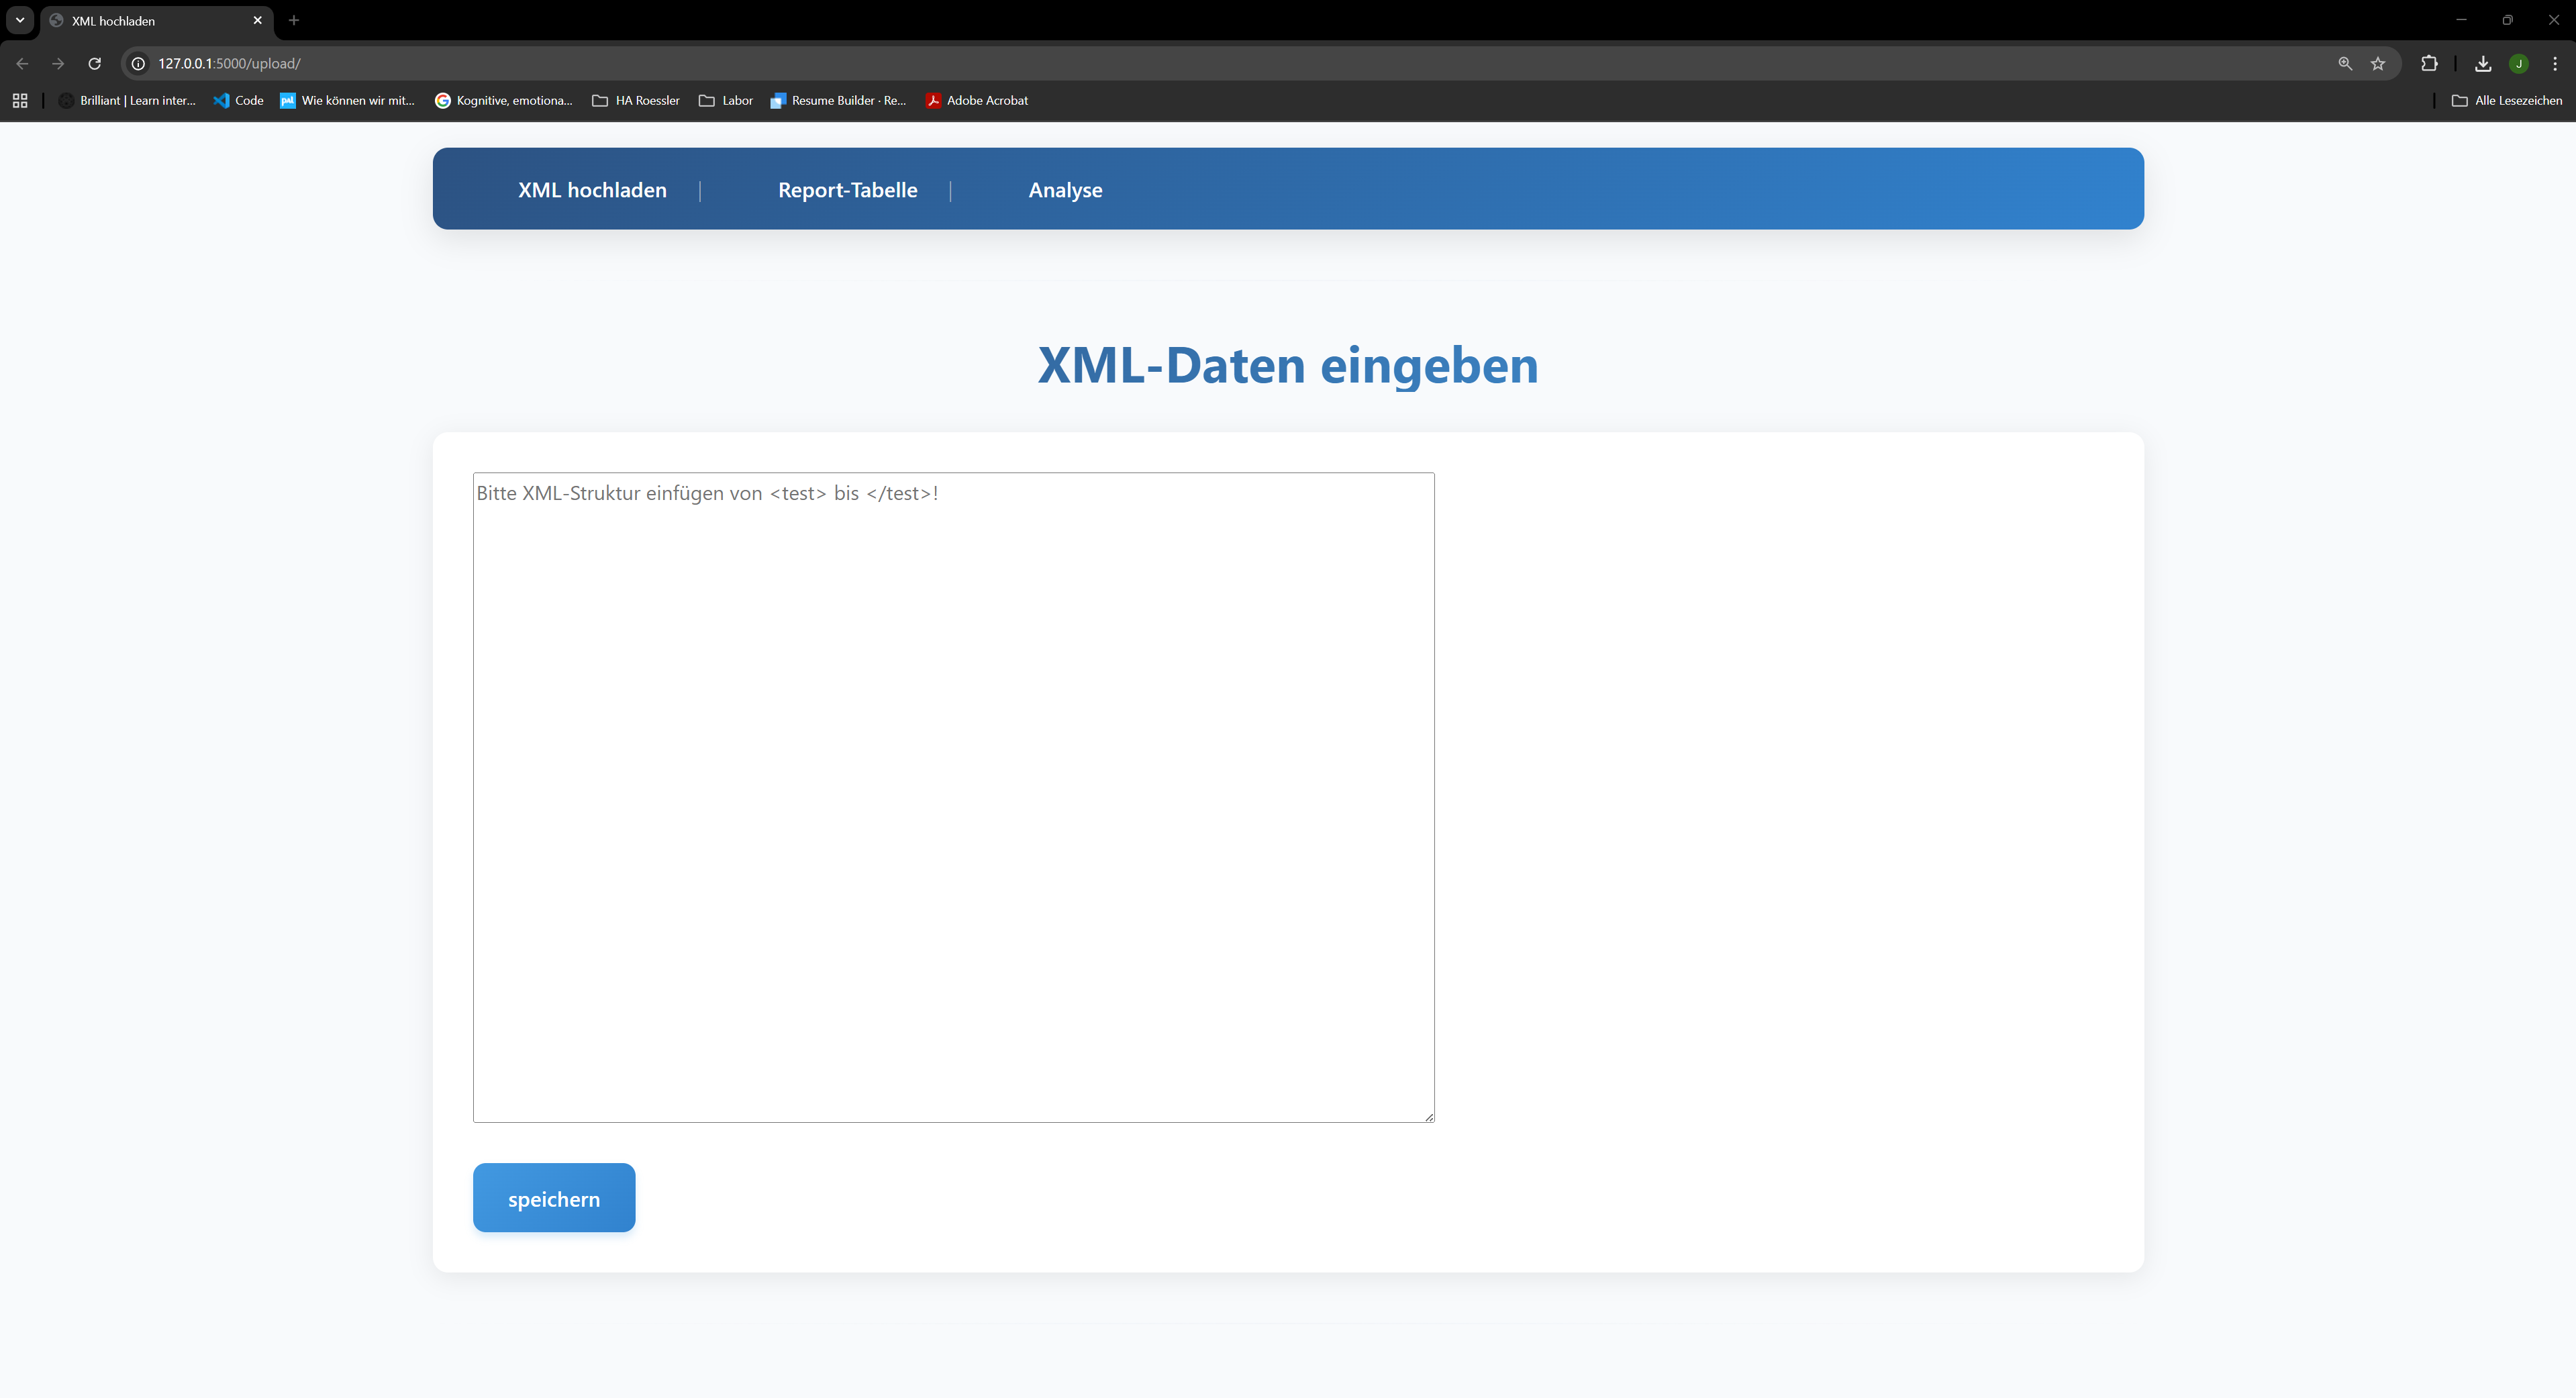
\includegraphics[width=1\textwidth]{Grafiken/Bild XML hochladen.png}
    \caption{Grundlegende Struktur des Applikations-Ordners}
    \label{fig: 4545}
    {Quelle: Eigene Darstellung mit Microsoft Visio}
\end{figure}

2. Report-Tabelle (\code{reports.html}): Übersicht aller eingelesenen Testberichte in Tabelle.
Die Seite ist in der folgenden Abbildung \ref{} dargestellt.

\begin{figure}[H]
    \centering
    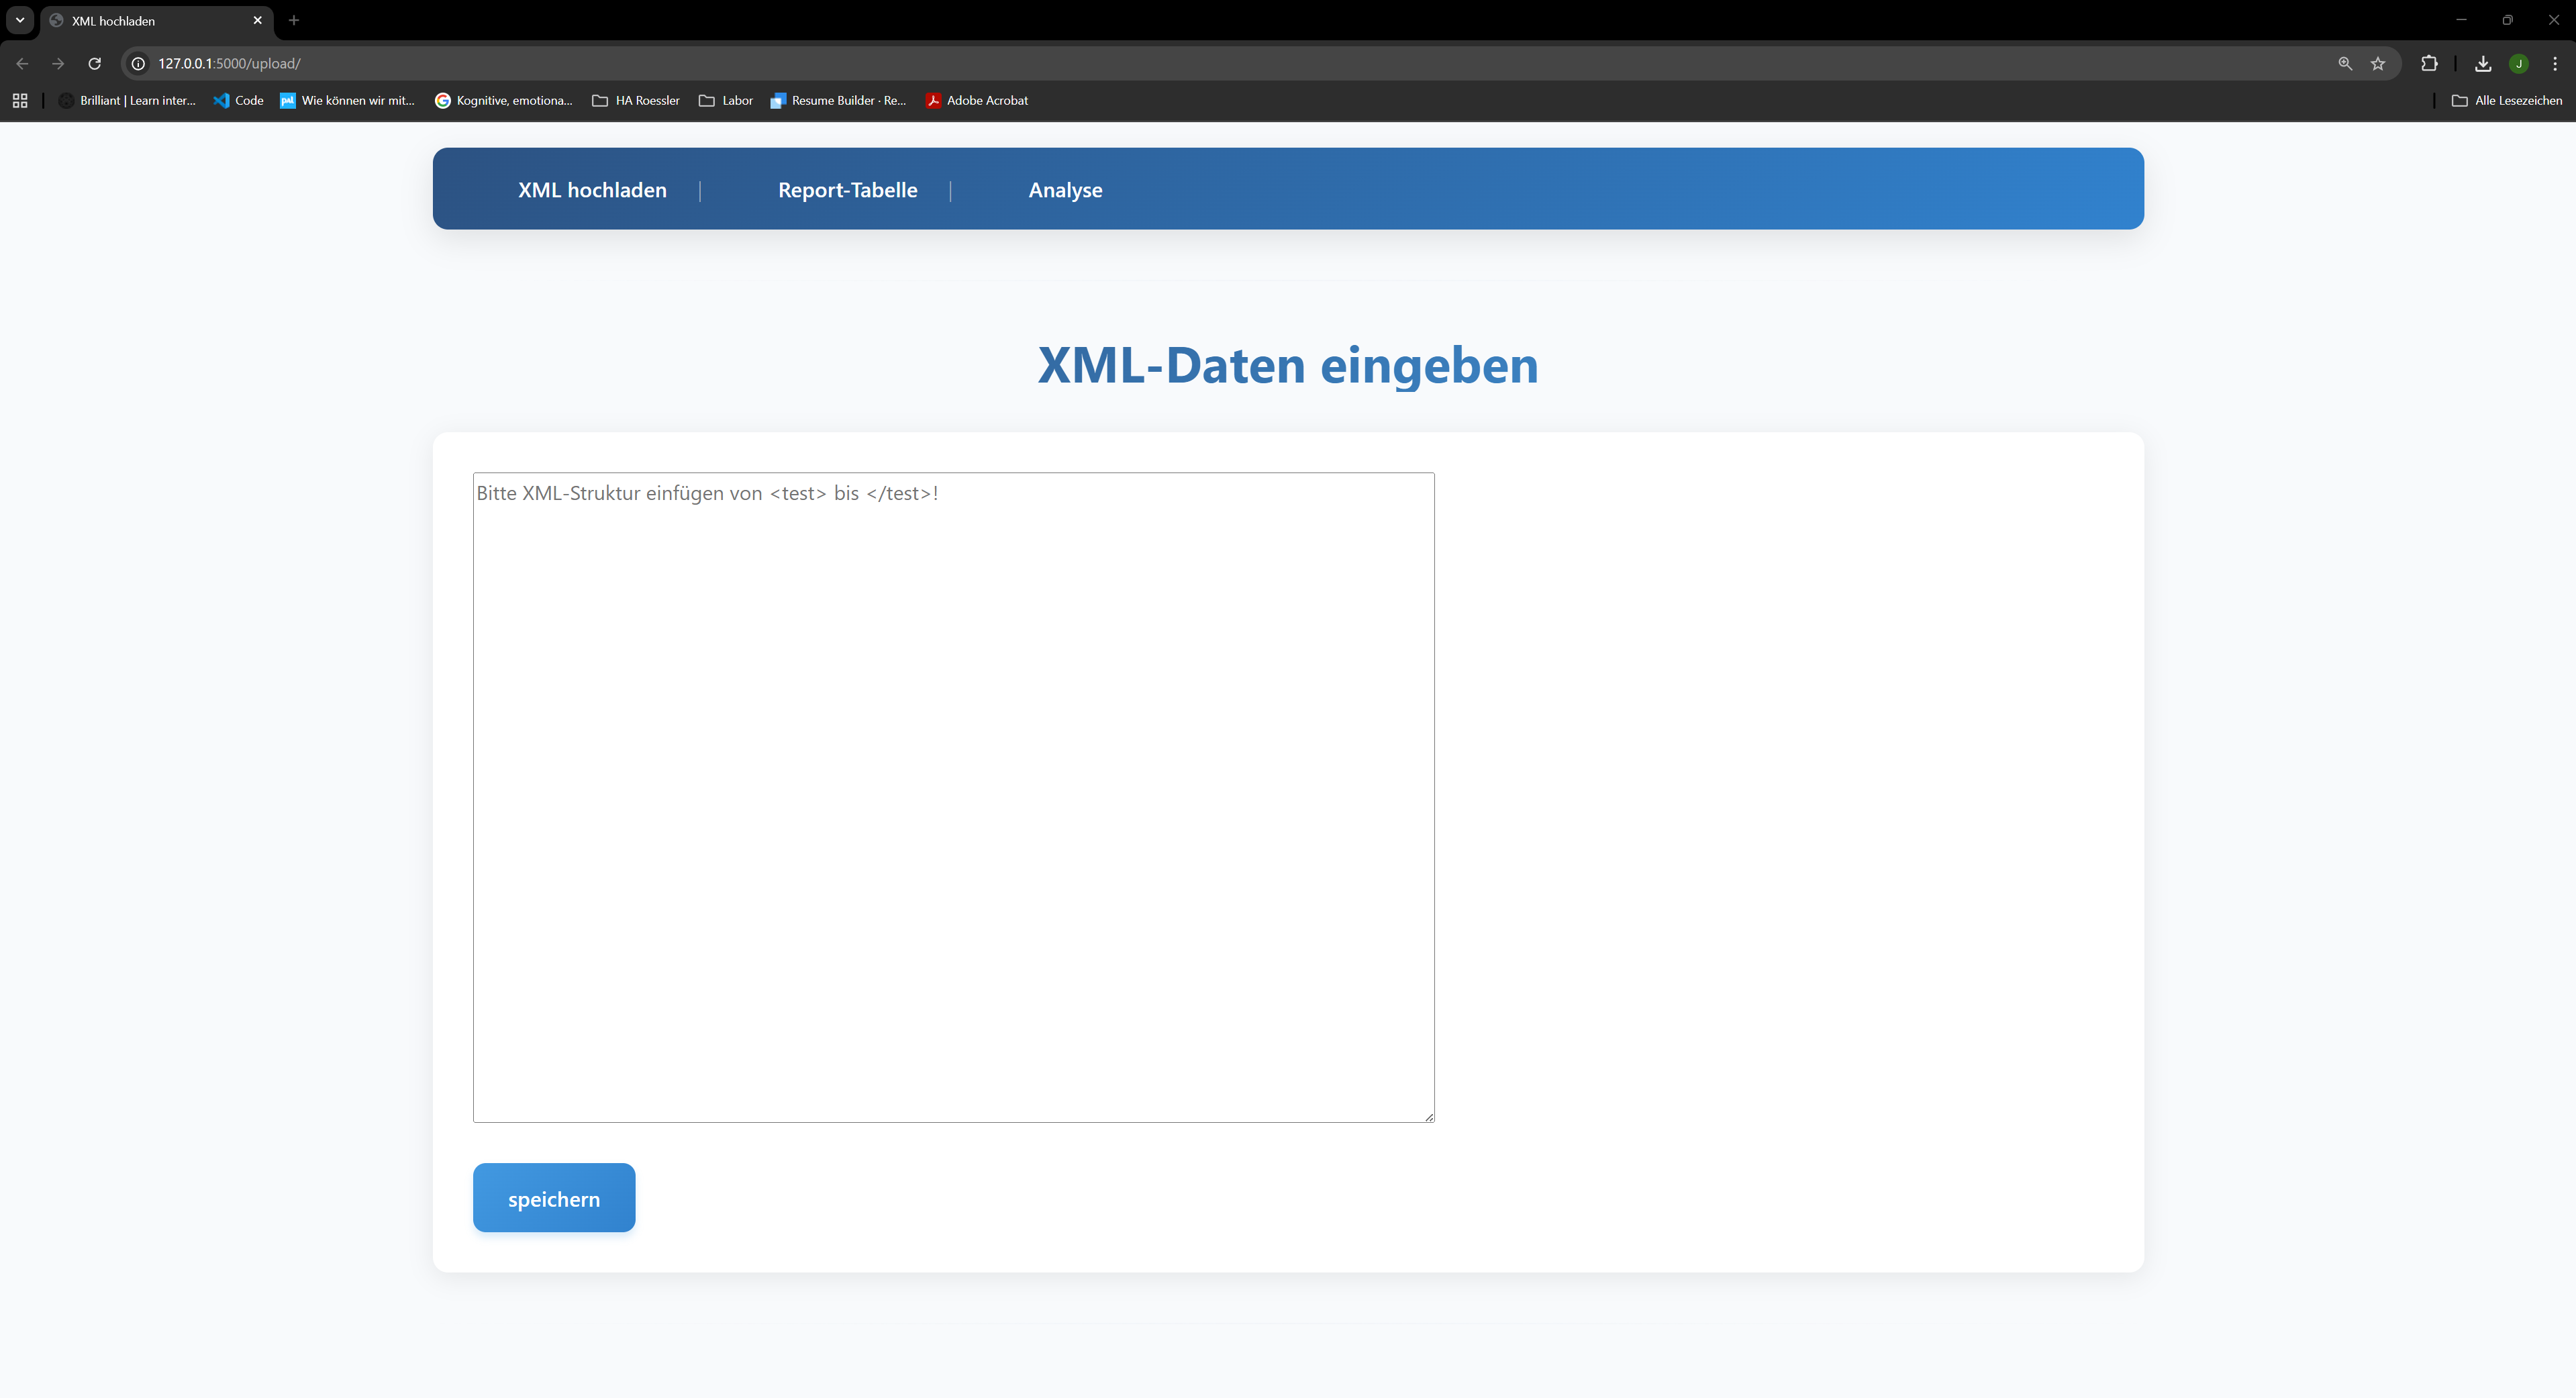
\includegraphics[width=1\textwidth]{Grafiken/Bild XML hochladen.png}
    \caption{Grundlegende Struktur des Applikations-Ordners}
    \label{fig: 343}
    {Quelle: Eigene Darstellung mit Microsoft Visio}
\end{figure}

3. Analyse (\code{dut\_analyse.html}): Darstellung ausgewählter Messdaten eines DUT aus einem Testbericht in grafischer Form.
Die Seite ist in der folgenden Abbildung \ref{} dargestellt.

\begin{figure}[H]
    \centering
    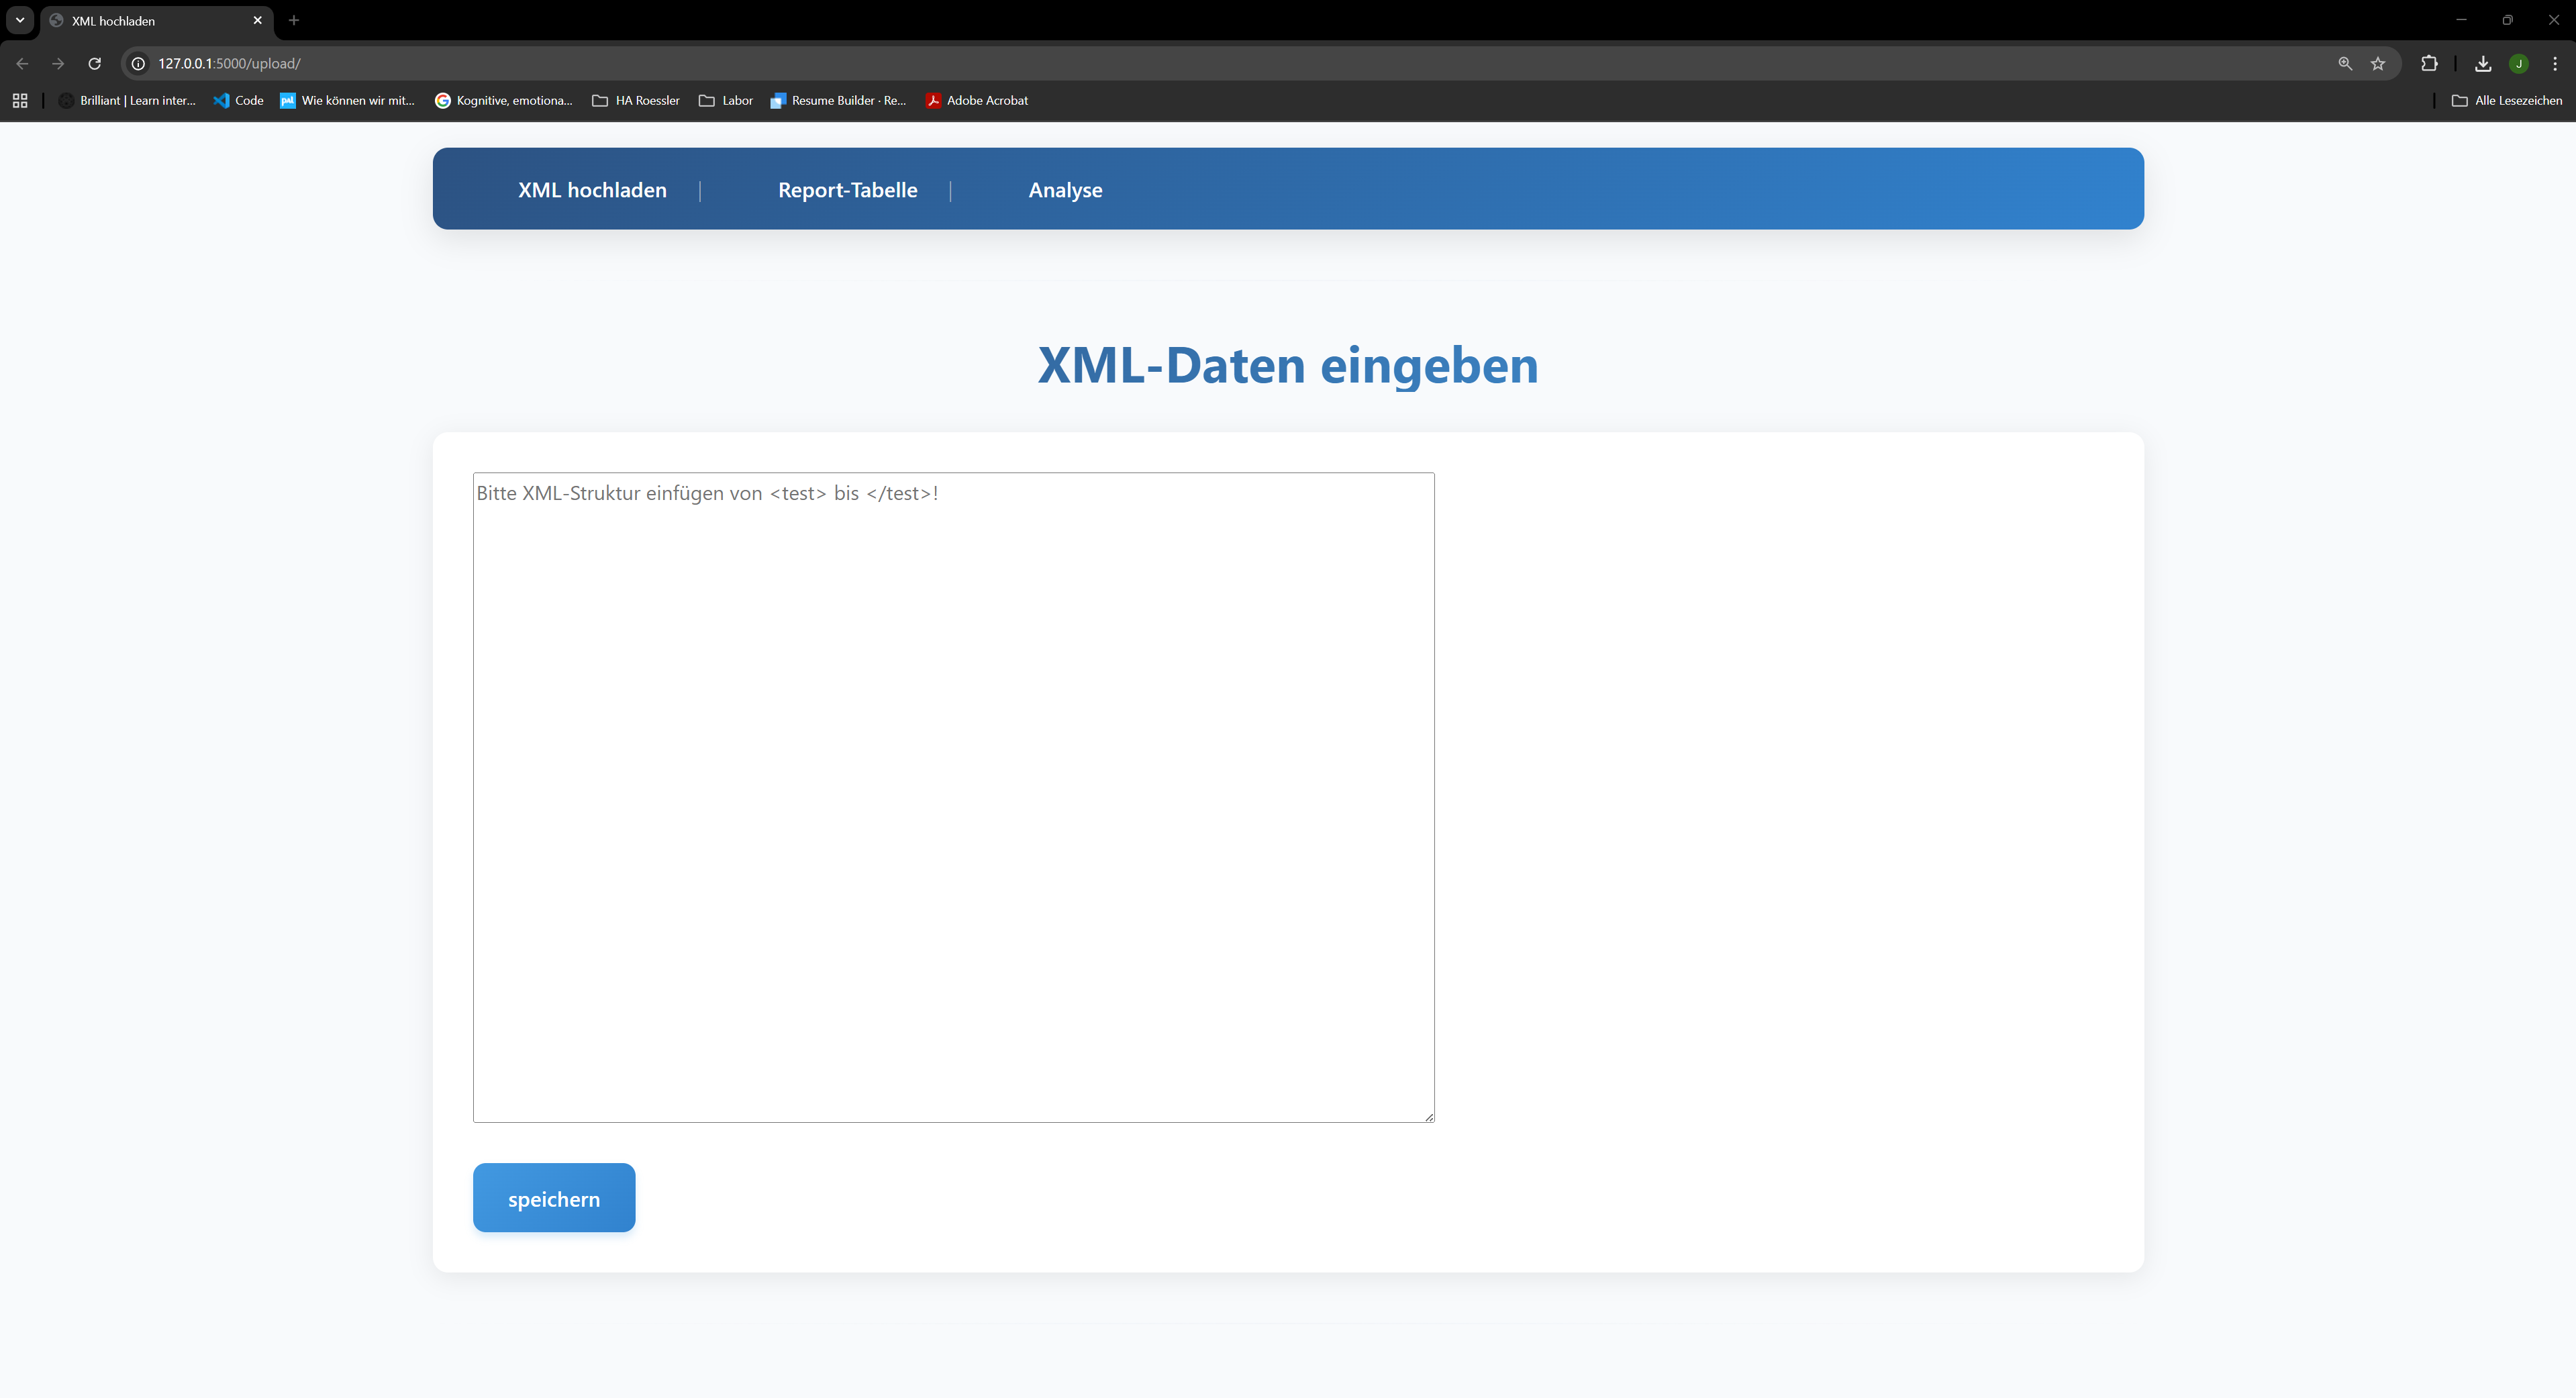
\includegraphics[width=1\textwidth]{Grafiken/Bild XML hochladen.png}
    \caption{Grundlegende Struktur des Applikations-Ordners}
    \label{fig: 12}
    {Quelle: Eigene Darstellung mit Microsoft Visio}
\end{figure}

Im Folgenden wird anhand der Beschreibung des Jinja2-Templates (\code{upload.html}) erläutert, wie die Übermittlung der Daten über einen Buttondruck an die Logikschicht abläuft.
Dieses Prinzip wird in allen Jinja2-Templates benutzt, um eingegebene Daten aus den Eingabefeldern der Webseite an die Logikschicht zu übermitteln.
Der Code aus \code{upload.html} ist in der Abbildung \ref{} für ein besseres Verständnis dargestellt.
Wie bereits oben schon genannt, erweitert das Template upload.html die in base.html definierte Grundstruktur und fügt deren allgemeine Elemente wie Navigationsleiste, Kopfbereich und Mitteilungsfeld ein.
Innerhalb des Blocks content wird der seitenindividuelle Inhalt definiert.
Hierzu gehört ein Eingabefeld in Form eines HTML-Formulars, das zur Eingabe der XML-Struktur dient.
Das Formular verwendet die Methode POST, wodurch die eingegebenen Daten an die Serverlogik gesendet werden, sobald der Benutzer den Button \textit{„speichern“} betätigt.
Über das csrf\_token-Feld wird ein Sicherheitsmechanismus implementiert, der Cross-Site-Request-Forgery-Angriffe verhindert.
Der eigentliche Eingabebereich wird durch ein <textarea>-Element realisiert, das genügend Platz bietet, um den XML-Inhalt – beginnend mit dem Stammelement <test> bis zum schließenden </test> – vollständig einzufügen.
Beim Betätigen des Buttons wird der Inhalt des Textfeldes an die zugehörige Flask-Route übergeben, wo die Daten serverseitig verarbeitet werden.
Die Applikationslogik übernimmt anschließend das Einlesen, Validieren und Speichern der XML-Struktur in der Datenbank.
Auf diese Weise wird eine direkte Verbindung zwischen der Benutzereingabe in der grafischen Oberfläche und der internen Verarbeitungsschicht hergestellt.
Die Implementierung zeigt beispielhaft, wie durch den Einsatz der Jinja2-Template-Engine eine klare Trennung zwischen Darstellungsebene (Frontend) und Logikebene (Backend) realisiert werden kann.
Das Template dient somit als Schnittstelle zwischen Benutzer und Anwendung und stellt sicher, dass Benutzereingaben strukturiert, sicher und nachvollziehbar an die Applikationslogik übergeben werden.
Dieses Prinzip findet sich in ähnlicher Form auch in den anderen Templates der Applikation wieder, wodurch eine einheitliche und konsistente Interaktion zwischen Benutzeroberfläche und Logikschicht gewährleistet wird.





